% Legacy line-like patterns only (easy visual diff).
\usetikzlibrary{patterns}

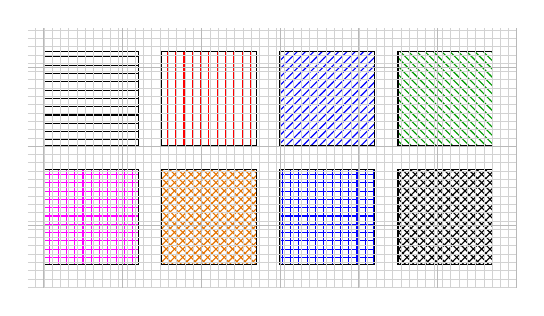
\begin{tikzpicture}[x=1cm,y=1cm]
  \path[draw,pattern=horizontal lines,pattern color=black] (0,0) rectangle +(1.2,1.2);
  \path[draw,pattern=vertical lines,pattern color=red] (1.5,0) rectangle +(1.2,1.2);
  \path[draw,pattern=north east lines,pattern color=blue] (3.0,0) rectangle +(1.2,1.2);
  \path[draw,pattern=north west lines,pattern color=green!60!black] (4.5,0) rectangle +(1.2,1.2);

  \path[draw,pattern=grid,pattern color=magenta] (0,-1.5) rectangle +(1.2,1.2);
  \path[draw,pattern=crosshatch,pattern color=orange!90!black] (1.5,-1.5) rectangle +(1.2,1.2);
  \path[draw,pattern={grid},pattern color=blue] (3.0,-1.5) rectangle +(1.2,1.2);
  \path[draw,pattern={crosshatch},pattern color=black] (4.5,-1.5) rectangle +(1.2,1.2);

  % Overlay reference grid for easier phase/offset comparison.
  \draw[step=3pt,gray!35,line width=.1pt] (-0.2,-1.8) grid (6.0,1.5);
  \draw[step=1cm,gray!55,line width=.16pt] (-0.2,-1.8) grid (6.0,1.5);
\end{tikzpicture}
